\documentclass[11pt]{article}

\usepackage[margin=1in]{geometry}
\usepackage{amsmath,amssymb,bm}
\usepackage{graphicx}
\usepackage{booktabs}
\usepackage{array}
\usepackage{xcolor}
\usepackage{microtype}
\usepackage{float}
\usepackage{enumitem}
\usepackage{hyperref}

\hypersetup{
  colorlinks=true,
  linkcolor=blue!45!black,
  citecolor=blue!45!black,
  urlcolor=blue!45!black,
  pdftitle={Density Matrices and Quantum Communication at Nonzero Spin-Orbit Coupling},
  pdfsubject={Helicity-resolved BdG conditional two-qubit states}
}

\newcommand{\SO}{V_{\mathrm{SO}}}
\newcommand{\bs}{\boldsymbol}
\newcommand{\tr}{\operatorname{Tr}}
\newcommand{\sgn}{\operatorname{sgn}}
\newcommand{\dd}{\mathrm d}
\newcommand{\Fbar}{\overline{\mathcal F}}
\newcommand{\kb}{\mathbf k}
\newcommand{\rr}{\mathbf r}
\allowdisplaybreaks
\newcommand{\SpinChiZero}{0.000007821}
\newcommand{\BandChiZero}{0.000003142}
\newcommand{\SpinChiNonzero}{0.000013593}
\newcommand{\BandChiNonzero}{0.002351021}
\newcommand{\SpinFrefNonzero}{0.500934644}
\newcommand{\SpinFoptNonzero}{0.501254157}
\newcommand{\BandFrefNonzero}{0.499739591}
\newcommand{\BandFoptNonzero}{0.500302714}
\newcommand{\SpinFefNonzero}{0.251881235}
\newcommand{\BandFefNonzero}{0.250454072}
\newcommand{\SpinSingletNonzero}{0.251401965}
\newcommand{\BandSingletNonzero}{0.249609387}


\title{\textbf{Density Matrices and Quantum Communication\\at Nonzero Spin--Orbit Coupling}\\[0.5em]
\large Conditional spin and helicity-pseudospin states in the Hubbard--Rashba BdG model}
\author{Technical derivation and validated numerical demonstration}
\date{\today}

\begin{document}
\maketitle

\begin{abstract}
\noindent
This report explains how to construct a two-qubit density matrix when the Rashba coupling $\SO$ is nonzero. The central change from the zero-SOC Oh--Kim construction is that scalar normal and anomalous correlations are no longer sufficient. One must retain $2\times2$ correlator matrices, transform the helicity pairing with the correct momentum-dependent spinors and gap phase, apply Wick's theorem, and only then normalize the sector containing one detected electron at each of two positions. The resulting original-spin state is generally neither an $X$ state nor a Werner state. A helicity-band calculation is also possible, but it describes helicity-pseudospin qubits whose local modes and operations are not automatically physical spin qubits and spin operations. We derive general concurrence, fixed-reference and optimized average teleportation fidelities, and the equal-probability Pauli-ensemble Holevo quantity used for dense coding. A separately archived $101\times101$ demonstration at $\SO/t=0$ and $0.5$ validates the construction: the zero-SOC Oh--Kim matrix is recovered to $5.55\times10^{-17}$, all 24 conditional matrices pass normalization and positivity checks, and the dense-coding implementation agrees with the repository's independent Holevo routine to $2.22\times10^{-16}$. The nonzero-SOC example is a methodological demonstration, not a converged SOC-dependence study or a claim of experimental helicity Bell measurement.
\end{abstract}

\tableofcontents
\clearpage

\section{Executive overview}
\label{sec:overview}

At $\SO=0$, the two helicity branches are degenerate and the original spin basis supports the Oh--Kim assumptions: spin-diagonal normal propagation and spin-singlet anomalous propagation. These assumptions lead to an $X$ state and, for the conditional two-spin reduction used here, a Werner state.

At $\SO\neq0$, spin and momentum are locked. The original-spin normal correlator can acquire off-diagonal components, while the pair correlator contains mixed singlet--triplet structure. Consequently, the correct generalization is not a new scalar $g(\rr),f(\rr)$ formula. It is the matrix contraction
\begin{equation}
\boxed{
\widetilde\rho_{\alpha\beta,\alpha'\beta'}
=
N_{B,\beta'\beta}N_{A,\alpha'\alpha}
-N_{BA,\beta'\alpha}N_{AB,\alpha'\beta}
+F_{AB,\alpha'\beta'}^{*}F_{AB,\alpha\beta}
}
\label{eq:headline}
\end{equation}
followed by $\rho_{AB}=\widetilde\rho_{AB}/\tr\widetilde\rho_{AB}$. The three terms are the direct, normal-exchange, and anomalous-pair contributions.

The following distinction governs every quantum-information interpretation in this report.
\begin{center}
\small
\begin{tabular}{p{0.22\textwidth}p{0.32\textwidth}p{0.36\textwidth}}
\toprule
Choice & Internal qubit states & Operational meaning \\
\midrule
Original spin & $\uparrow,\downarrow$ at $A,B$ & Ordinary spin entanglement and spin protocols; generally a non-$X$, non-Werner state at nonzero SOC. \\
Helicity band & $s=+1,-1$ at band-filtered modes & Band-pseudospin entanglement and protocols; requires band-pseudospin local unitaries, Bell measurement, and feedforward. \\
\bottomrule
\end{tabular}
\end{center}

The demonstration finds ideal singlets at zero separation, but no concurrence, teleportation advantage, or dense-coding advantage at the tested nonzero lattice vectors for either basis. This is a limited numerical observation at one mesh and parameter set, not a general theorem about Rashba superconductors.

\section{Model, symmetries, and the meaning of helicity}
\label{sec:model}

The square-lattice normal-state dispersion is
\begin{equation}
\epsilon_{\kb s}
=-2t(\cos k_x+\cos k_y)-2s\SO\lambda_{\kb},
\qquad
\lambda_{\kb}=\sqrt{\sin^2k_x+\sin^2k_y},
\label{eq:dispersion}
\end{equation}
with $s=\pm1$. The BdG quasiparticle energy and zero-temperature occupation are
\begin{equation}
E_{\kb s}=\sqrt{(\epsilon_{\kb s}-\mu)^2+|\Delta_{\kb s}|^2},
\qquad
v_{\kb s}^2=\frac12\left(1-\frac{\epsilon_{\kb s}-\mu}{E_{\kb s}}\right).
\label{eq:energy}
\end{equation}
The self-consistency equations determine $\Delta_0,\Delta_S,\mu$ anew for each SOC and filling. A converged stationary solution is required before any density matrix is computed; a residual check alone, however, does not establish global thermodynamic stability.

\subsection{What changes when $\SO$ is turned on?}

At zero SOC, spin rotational symmetry makes the original spin basis natural. At nonzero SOC, the normal Hamiltonian is diagonal in a helicity basis whose spin quantization axis depends on $\kb$. Helicity is therefore a useful band quantum number, but it is not a single global spin projection shared by all momenta.

This has three distinct consequences:
\begin{enumerate}[label=(\roman*)]
\item original-spin normal correlations need not be diagonal;
\item time-reversed intraband pairing transforms into mixed original-spin singlet--triplet correlations;
\item an on-site ``helicity qubit'' is not unique unless the band-filtered modes are explicitly defined.
\end{enumerate}
None of these statements makes original-spin entanglement undefined. Entanglement is a property of a state \emph{and a tensor-product decomposition}. One may choose original-spin modes or helicity-band modes, but the two choices define different resources.

\section{Helicity transformation and full pairing phase}
\label{sec:helicity}

Hutchinson, Hirsch, and Marsiglio define~\cite{Hutchinson2018}
\begin{equation}
c_{\kb s}^{\dagger}
=\frac{c_{\kb\uparrow}^{\dagger}+s e^{i\theta_{\kb}}c_{\kb\downarrow}^{\dagger}}{\sqrt2},
\qquad
e^{i\theta_{\kb}}=\frac{\sin k_y-i\sin k_x}{\lambda_{\kb}}.
\label{eq:helicity_operators}
\end{equation}
Inverting the transformation gives $c_{\kb\sigma}=\sum_s U_{\kb,\sigma s}c_{\kb s}$ with
\begin{equation}
U_{\kb}=\frac1{\sqrt2}
\begin{pmatrix}
1&1\\
e^{i\theta_{\kb}}&-e^{i\theta_{\kb}}
\end{pmatrix},
\qquad U_{-\kb}=ZU_{\kb},\quad Z=\operatorname{diag}(1,-1),
\label{eq:spinors}
\end{equation}
because $e^{i\theta_{-\kb}}=-e^{i\theta_{\kb}}$.

The mean field pairs time-reversed electrons within the same helicity band. Its full gap is
\begin{equation}
\boxed{\Delta_{\kb s}=s e^{-i\theta_{\kb}}\bar\Delta_{\kb s}.}
\label{eq:full_gap}
\end{equation}
The repository's \verb|bdg["Delta_ks"]| stores the even scalar $\bar\Delta_{\kb s}$. Omitting the phase in Eq.~\eqref{eq:full_gap} destroys the correct relation between $\kb$ and $-\kb$ and can produce spurious same-band pairing.

At $T=0$, the pair mean field satisfies $b_{\kb s}=\bar\Delta_{\kb s}/(2E_{\kb s})$. Up to one common sign that cancels from $F^*F$, define
\begin{align}
N^{\mathrm h}_{\kb}
&=\begin{pmatrix}v_{\kb +}^2&0\\0&v_{\kb -}^2\end{pmatrix},
\label{eq:Nband}\\
F^{\mathrm h}_{\kb}
&=\begin{pmatrix}
e^{-i\theta_{\kb}}\bar\Delta_{\kb +}/(2E_{\kb +})&0\\
0&-e^{-i\theta_{\kb}}\bar\Delta_{\kb -}/(2E_{\kb -})
\end{pmatrix}.
\label{eq:Fband}
\end{align}
Here $N_{\kb,ss'}=\langle c_{\kb s}^{\dagger}c_{\kb s'}\rangle$ and $F_{\kb,ss'}=\langle c_{\kb s}c_{-\kb s'}\rangle$.

\subsection{TRIM and Pauli exclusion}

At a time-reversal-invariant momentum (TRIM), $\lambda_{\kb}=0$ and the helicity phase is singular. For nondegenerate same-band pairing, $c_{\kb s}$ and $c_{-\kb s}$ coincide up to a gauge, so the pair amplitude must vanish by Pauli exclusion. The implementation enforces this at TRIM points. At exact zero-SOC degeneracy, the original-spin singlet is instead gauge invariant and is treated separately.

Off a TRIM, the full phase gives
\begin{equation}
F^{\mathrm h}_{-\kb}=-F^{\mathrm h}_{\kb}.
\label{eq:inversion}
\end{equation}
The numerical maximum off-TRIM residual in Eq.~\eqref{eq:inversion} is $3.30\times10^{-15}$.

\section{Matrix-valued correlators}
\label{sec:correlators}

\subsection{Transforming back to original spin}

For the creation--annihilation convention $N_{\sigma\sigma'}=\langle c_\sigma^\dagger c_{\sigma'}\rangle$, the correct transformations are
\begin{equation}
\boxed{
N^{\mathrm{spin}}_{\kb}=U_{\kb}^{*}N^{\mathrm h}_{\kb}U_{\kb}^{T},
\qquad
F^{\mathrm{spin}}_{\kb}=U_{\kb}F^{\mathrm h}_{\kb}U_{-\kb}^{T}.
}
\label{eq:spin_transform}
\end{equation}
The first expression is not $UNU^\dagger$ under this index convention. Direct multiplication confirms the phase of $\langle c_\uparrow^\dagger c_\downarrow\rangle$. The anomalous transformation uses both $U_{\kb}$ and $U_{-\kb}$ because the two electrons have opposite momenta.

At zero SOC, the two bands are degenerate and Eq.~\eqref{eq:spin_transform} restores a scalar normal matrix and a singlet anomalous matrix. At nonzero SOC, the normal matrix can have off-diagonal elements and the anomalous matrix can contain both singlet and triplet structures.

\subsection{Fourier transformation to two positions}

Let $A,B$ be lattice positions and $\rr=\mathbf R_B-\mathbf R_A$. For either basis,
\begin{equation}
N_{AB}(\rr)=\frac1{N_k^2}\sum_{\kb}e^{i\kb\cdot\rr}N_{\kb},
\qquad
F_{AB}(\rr)=\frac1{N_k^2}\sum_{\kb}e^{-i\kb\cdot\rr}F_{\kb}.
\label{eq:real_space}
\end{equation}
Uniformity gives $N_A=N_B=N_{AB}(0)$ and $N_{BA}=N_{AB}^{\dagger}$. Direct anticommutation at the same ordered positions gives
\begin{equation}
F_{BA,\beta\alpha}=\langle c_{B\beta}c_{A\alpha}\rangle=-F_{AB,\alpha\beta}.
\label{eq:FBA}
\end{equation}
At $A=B$, $F_{AB}(0)=-F_{AB}^{T}(0)$ exactly. The code removes only the finite-quadrature symmetric residue at this point. It does not repair an unphysical state by clipping eigenvalues.

\section{Conditional Wick construction of the density matrix}
\label{sec:wick}

\subsection{Detection sector}

The full BCS state contains variable particle number. A two-qubit communication resource is defined only after selecting the sector with one electron detected at $A$ and one at $B$. This is the same conditional logic as the Oh--Kim reduction, but without assuming scalar spin propagation.

For a Gaussian BdG mean-field state, Wick's theorem gives
\begin{align}
\widetilde\rho_{\alpha\beta,\alpha'\beta'}
&=\langle c_{B\beta'}^{\dagger}c_{A\alpha'}^{\dagger}
 c_{A\alpha}c_{B\beta}\rangle\nonumber\\
&=N_{B,\beta'\beta}N_{A,\alpha'\alpha}
-N_{BA,\beta'\alpha}N_{AB,\alpha'\beta}
+F_{AB,\alpha'\beta'}^{*}F_{AB,\alpha\beta}.
\label{eq:wick_full}
\end{align}
The basis ordering is $\{|00\rangle,|01\rangle,|10\rangle,|11\rangle\}$. The normalized matrix and detection-sector weight are
\begin{equation}
P_{AB}=\tr\widetilde\rho_{AB},
\qquad
\rho_{AB}=\frac{\widetilde\rho_{AB}}{P_{AB}}.
\label{eq:normalization}
\end{equation}
The weight is retained in the output. It should not be confused with a communication fidelity.

The creation-side anomalous factor is $F_{AB,\alpha'\beta'}^*$, equivalently $-F_{BA,\beta'\alpha'}^*$. This sign is essential: it produces the negative singlet coherence and the exact zero-SOC limit.

\subsection{Why the result is a valid state}

The unnormalized matrix is a projected positive two-detection operator. Therefore, for a physical Gaussian input state and exact arithmetic,
\begin{equation}
\widetilde\rho_{AB}=\widetilde\rho_{AB}^{\dagger},
\qquad \widetilde\rho_{AB}\geq0,
\qquad P_{AB}>0.
\end{equation}
After normalization, $\rho_{AB}$ is Hermitian, positive semidefinite, and has unit trace. These properties are checked numerically rather than assumed from a target $X$-matrix form.

At $A=B$, Pauli exclusion leaves only the antisymmetric internal state, so the conditional matrix is the same-site singlet. The test recovers it to $1.11\times10^{-16}$ in both bases.

\section{Exact recovery of the zero-SOC Oh--Kim state}
\label{sec:ohkim_section}

The Oh--Kim reduction~\cite{Oh2005} follows when

\begin{equation}
N_A=N_B=n_0I,\qquad N_{AB}=N_{BA}=n_0g(\rr)I,
\qquad F_{AB}=n_0f(\rr)i\sigma_y.
\end{equation}
Then Eq.~\eqref{eq:wick_full} reduces to
\begin{equation}
\rho_X=\frac1{\mathcal N}
\begin{pmatrix}
1-g^2&0&0&0\\
0&1+f^2&-(g^2+f^2)&0\\
0&-(g^2+f^2)&1+f^2&0\\
0&0&0&1-g^2
\end{pmatrix},
\label{eq:ohkim}
\end{equation}
where $g^2=|g|^2$, $f^2=|f|^2$, and $\mathcal N=4-2g^2+2f^2$. Defining
\begin{equation}
w=\frac{g^2+f^2}{2+f^2-g^2},
\qquad
|\Psi^-\rangle=\frac{|01\rangle-|10\rangle}{\sqrt2},
\end{equation}
gives the Werner representation
\begin{equation}
\rho_X=(1-w)\frac{I_4}{4}+w|\Psi^-\rangle\langle\Psi^-|.
\label{eq:werner}
\end{equation}
This special structure explains why fixed and optimized teleportation formulas coincide in the earlier $V_{\mathrm{SO}}=0$ study. It must not be imposed at nonzero SOC.

The implementation recovers Eq.~\eqref{eq:ohkim} with maximum elementwise error $5.55\times10^{-17}$ in the executed zero-SOC test.

\section{Spin qubits versus helicity-pseudospin qubits}
\label{sec:qubits}

\subsection{Original-spin modes}

For \verb|basis="spin"|, the internal states are the original $\uparrow,\downarrow$ modes at $A,B$. This is the appropriate construction for ordinary spin entanglement and spin teleportation. Nonzero SOC changes the state but not the definition of these local spin modes.

\subsection{Band-lattice modes}

For \verb|basis="band"|, the implementation uses
\begin{equation}
d_{i,s}=\frac1{N_k}\sum_{\kb}e^{i\kb\cdot\mathbf R_i}c_{\kb s}.
\label{eq:band_modes}
\end{equation}
These are canonical fermionic modes and therefore define a valid mathematical qubit basis after conditional detection. They are, however, nonlocal combinations of original spin/site modes. The corresponding band-pseudospin singlet is not generally the original-spin singlet.

Because the helicity transformation depends on momentum, the original-spin and band-lattice states are not related by a fixed pair of local spin rotations. Their concurrences, entropies, and communication benchmarks can differ. This is not a numerical contradiction; it is a change of tensor-product decomposition and operational resource.

\subsection{Operational assumptions}

For helicity-pseudospin teleportation, one must assume independently addressable $A,B$ band modes, an independently prepared input pseudospin $Q$, ideal band-basis Bell measurement on $Q,A$, and ideal classical feedforward to $B$. For helicity-pseudospin dense coding, one must similarly implement band-pseudospin Pauli encodings, transmit the encoded band mode, and perform joint decoding.

The calculation does not establish microscopic Bell-measurement feasibility, individual Cooper-pair addressability, or an experimental band-filter implementation. For ordinary physical spin protocols, the original-spin basis is the unambiguous choice.

\section{Entanglement at nonzero SOC}
\label{sec:entanglement}

The generalized state need not be an $X$ state. Concurrence is therefore calculated using Wootters' general two-qubit formula~\cite{Wootters1998}:
\begin{equation}
R=(\sigma_y\otimes\sigma_y)\rho_{AB}^{*}(\sigma_y\otimes\sigma_y),
\end{equation}
\begin{equation}
C(\rho_{AB})=\max\{0,\lambda_1-\lambda_2-\lambda_3-\lambda_4\},
\label{eq:concurrence}
\end{equation}
where $\lambda_i$ are the decreasingly ordered square roots of the eigenvalues of $\rho_{AB}R$. In the band calculation, $\sigma_y$ acts on band pseudospin.

Several quantities must not be conflated:
\begin{itemize}
\item a large anomalous correlator $F$ is not itself concurrence;
\item a nonzero superconducting gap does not guarantee finite-site entanglement;
\item zero concurrence does not imply zero singlet overlap or zero Holevo quantity;
\item concurrence in the original-spin basis need not equal concurrence in the band-pseudospin basis.
\end{itemize}

The zero-separation conditional state has $C=1$. At every tested nonzero lattice vector in the demonstration, $C=0$ for both bases. This statement is limited to the reported parameter set and mesh.

\section{Teleportation fidelity}
\label{sec:teleportation}

\subsection{Fixed Bell-reference protocol}

Let $F_{\mathrm h}=\langle\Psi^-_{\mathrm h}|\rho_{AB}|\Psi^-_{\mathrm h}\rangle$ be the overlap with the chosen reference Bell state in the same qubit basis. For the fixed protocol referenced to that state, the average over uniformly distributed pure input qubits is~\cite{Bennett1993,Horodecki1999}
\begin{equation}
\Fbar_{\mathrm{ref}}=\frac{2F_{\mathrm h}+1}{3}.
\label{eq:fixed_tel}
\end{equation}
The reference overlap is not automatically the fully entangled fraction.

\subsection{Locally optimized protocol}

Define the real correlation matrix
\begin{equation}
T_{ij}=\tr[\rho_{AB}(\sigma_i\otimes\sigma_j)].
\end{equation}
The fully entangled fraction, optimized over local single-qubit unitaries, is
\begin{equation}
\mathfrak f=\max_{U_A,U_B}\langle\Phi^+|(U_A\otimes U_B)\rho_{AB}(U_A\otimes U_B)^\dagger|\Phi^+\rangle
=\frac{1+\sum_i\nu_i(T)}4,
\label{eq:fef}
\end{equation}
where $\nu_i(T)$ are singular values. The optimized average fidelity is
\begin{equation}
\Fbar_{\mathrm{opt}}=\frac{2\mathfrak f+1}{3}.
\label{eq:opt_tel}
\end{equation}
Consequently,
\begin{equation}
\Fbar_{\mathrm{opt}}>\frac23
\Longleftrightarrow \mathfrak f>\frac12
\Longleftrightarrow \sum_i\nu_i(T)>1.
\label{eq:classical_tel}
\end{equation}
Local optimization is performed in the selected spin or band-pseudospin basis. The latter assumes band-pseudospin local unitaries.

For a Werner state of weight $w$,
\begin{equation}
F_{\mathrm h}=\mathfrak f=\frac{1+3w}{4},
\qquad
\Fbar_{\mathrm{ref}}=\Fbar_{\mathrm{opt}}=\frac{1+w}{2}.
\end{equation}
For a general nonzero-SOC state, these identities need not hold.

At $\SO=0.5t$ and $\rr=(1,0)$, the original-spin example has
\begin{equation}
F_{\mathrm h}=\SpinSingletNonzero,\quad
\mathfrak f=\SpinFefNonzero,\quad
\Fbar_{\mathrm{ref}}=\SpinFrefNonzero,\quad
\Fbar_{\mathrm{opt}}=\SpinFoptNonzero.
\end{equation}
The band example instead has
\begin{equation}
F_{\mathrm h}=\BandSingletNonzero,\quad
\mathfrak f=\BandFefNonzero,\quad
\Fbar_{\mathrm{ref}}=\BandFrefNonzero,\quad
\Fbar_{\mathrm{opt}}=\BandFoptNonzero.
\end{equation}
Fixed and optimized fidelities differ, and all are far below $2/3$.

\section{Dense coding with SOC}
\label{sec:dense_coding}

\subsection{Protocol and Pauli ensemble}

Dense coding uses a shared $\rho_{AB}$, local encoding on $A$, transmission of $A$ to $B$, and joint decoding~\cite{BennettWiesner1992,Bruss2004}. The implemented ensemble applies $I,X,Y,Z$ on $A$ with equal probability. In a band calculation these are helicity-pseudospin Pauli operations.

The ensemble average is
\begin{equation}
\bar\rho_{AB}=\frac14\sum_{i=0}^{3}
(\sigma_i\otimes I)\rho_{AB}(\sigma_i\otimes I)^\dagger.
\end{equation}
The Pauli twirl identity gives, for any two-qubit state,
\begin{equation}
\bar\rho_{AB}=\frac{I_A}{2}\otimes\rho_B,
\qquad \rho_B=\tr_A\rho_{AB}.
\label{eq:pauli_twirl}
\end{equation}
Therefore the Holevo quantity of this ensemble is
\begin{equation}
\boxed{
\chi_{\mathrm P}
=S_2(\bar\rho_{AB})-S_2(\rho_{AB})
=1+S_2(\rho_B)-S_2(\rho_{AB}),
}
\label{eq:holevo}
\end{equation}
with base-two entropies. Its bounds are $0\leq\chi_{\mathrm P}\leq2$ bits. One bit is the classical one-qubit benchmark; values above one bit indicate an advantage for the stated ideal protocol.

This is the dense-coding capacity when the protocol is restricted to the specified Pauli encoding with ideal transmission and asymptotic joint decoding. It is not automatically a general optimization over all encodings, a one-shot accessible-information result, or an experimentally achieved communication rate.

\subsection{SOC and basis dependence}

SOC enters $\chi_{\mathrm P}$ through $\rho_{AB}$ and $\rho_B$. There is no universal rule that increasing SOC must increase or decrease dense coding. It can change both the total entropy and the reduced entropy.

The identity Eq.~\eqref{eq:holevo} is valid in either qubit basis. However, original-spin and helicity-band states need not be related by fixed local unitaries, so their numerical $\chi_{\mathrm P}$ values need not agree. At $\rr=(1,0)$,
\begin{equation}
\chi_{\mathrm P}^{\mathrm{spin}}(\SO=0)=\SpinChiZero,\qquad
\chi_{\mathrm P}^{\mathrm{band}}(\SO=0)=\BandChiZero,
\end{equation}
whereas at $\SO=0.5t$,
\begin{equation}
\chi_{\mathrm P}^{\mathrm{spin}}=\SpinChiNonzero,\qquad
\chi_{\mathrm P}^{\mathrm{band}}=\BandChiNonzero.
\end{equation}
The band value is larger in this particular example, but remains far below one bit. This is not evidence of a general SOC enhancement or an operational advantage.

Useful limiting checks are
\begin{equation}
\rho=|\Psi^-\rangle\langle\Psi^-|\Rightarrow\chi_{\mathrm P}=2,
\qquad
\rho=|00\rangle\langle00|\Rightarrow\chi_{\mathrm P}=1,
\qquad
\rho=I_4/4\Rightarrow\chi_{\mathrm P}=0.
\end{equation}
Thus the one-bit value of a pure product state is the classical benchmark, not a residual dense-coding advantage. Concurrence, teleportation fidelity, and Holevo information must be evaluated separately.

No new noisy dense-coding dynamics are generated in this report. If a spin or band-pseudospin channel is applied, the evolved state and its reduced entropy must be recomputed with the corresponding Kraus operators. The legacy original-spin amplitude-damping results must not be relabeled as helicity-band dynamics.

\section{Numerical demonstration and validation}
\label{sec:numerics}

\subsection{Parameters and solver checks}

The demonstration independently solves the self-consistency equations at $\SO/t=0$ and $0.5$ with
\begin{center}
\begin{tabular}{ll}
\toprule
Parameter & Value \\
\midrule
$U/t$ & 75 \\
$\Delta_t/t$ & 4.5 \\
Filling $n$ & 1.875 \\
Temperature & $T=0$ \\
Momentum mesh & $101\times101$, inversion symmetric \\
Lattice vectors & $(0,0),(1,0),(1,1),(2,0),(0,2),(3,1)$ \\
Bases & Original spin and helicity band \\
\bottomrule
\end{tabular}
\end{center}
The odd mesh includes paired $\kb,-\kb$ points, allowing exact inversion-cancellation checks. The calculation is not a production mesh-convergence or seed-stability study.

\begin{table}[H]
\centering
\small
\caption{Executed validation diagnostics. All checks passed.}
\begin{tabular}{lc}
\toprule
Diagnostic & Maximum absolute value \\
\midrule
Zero-SOC solver residual & $2.906e-12$ \\
Nonzero-SOC solver residual & $3.354e-12$ \\
Zero-SOC Oh--Kim matrix error & $5.551e-17$ \\
Trace error & $1.110e-16$ \\
Hermiticity error & $0.000e+00$ \\
Same-site singlet error & $1.110e-16$ \\
Off-TRIM anomalous inversion residual & $3.297e-15$ \\
Pauli-average identity error & $2.776e-17$ \\
Holevo repository cross-check & $2.220e-16$ \\
Bell/Werner metric error & $2.665e-15$ \\
Minimum density-matrix eigenvalue & $-1.564e-32$ \\
\bottomrule
\end{tabular}

\label{tab:validation}
\end{table}

\subsection{Explicit nonzero-SOC matrices}

The following matrices are generated directly from the validated NPZ file. The code retains full complex values; the displayed entries are real to the shown precision.
\begin{equation}
\rho_{\mathrm{spin}}(V_{\mathrm{SO}}=0.5t,\mathbf r=(1,0))
\approx
\begin{pmatrix}
0.24961259 & -0.00049305 & 0.00049305 & 0.00023973 \\
-0.00049305 & 0.25038741 & -0.00101455 & -0.00049305 \\
0.00049305 & -0.00101455 & 0.25038741 & 0.00049305 \\
0.00023973 & -0.00049305 & 0.00049305 & 0.24961259
\end{pmatrix},
\end{equation}

\begin{equation}
\rho_{\mathrm{band}}(V_{\mathrm{SO}}=0.5t,\mathbf r=(1,0))
\approx
\begin{pmatrix}
0.27889114 & 0.00000000 & 0.00000000 & 0.00008567 \\
0.00000000 & 0.24963159 & 0.00002221 & 0.00000000 \\
0.00000000 & 0.00002221 & 0.24963159 & 0.00000000 \\
0.00008567 & 0.00000000 & 0.00000000 & 0.22184567
\end{pmatrix}.
\end{equation}


The original-spin matrix contains elements outside the Oh--Kim $X$ pattern, including $|00\rangle\langle11|$ coherence and local-spin off-diagonal structure. The band matrix has a different diagonal and coherence structure. Forcing either matrix into the scalar Werner form would discard information.

\begin{figure}[H]
\centering
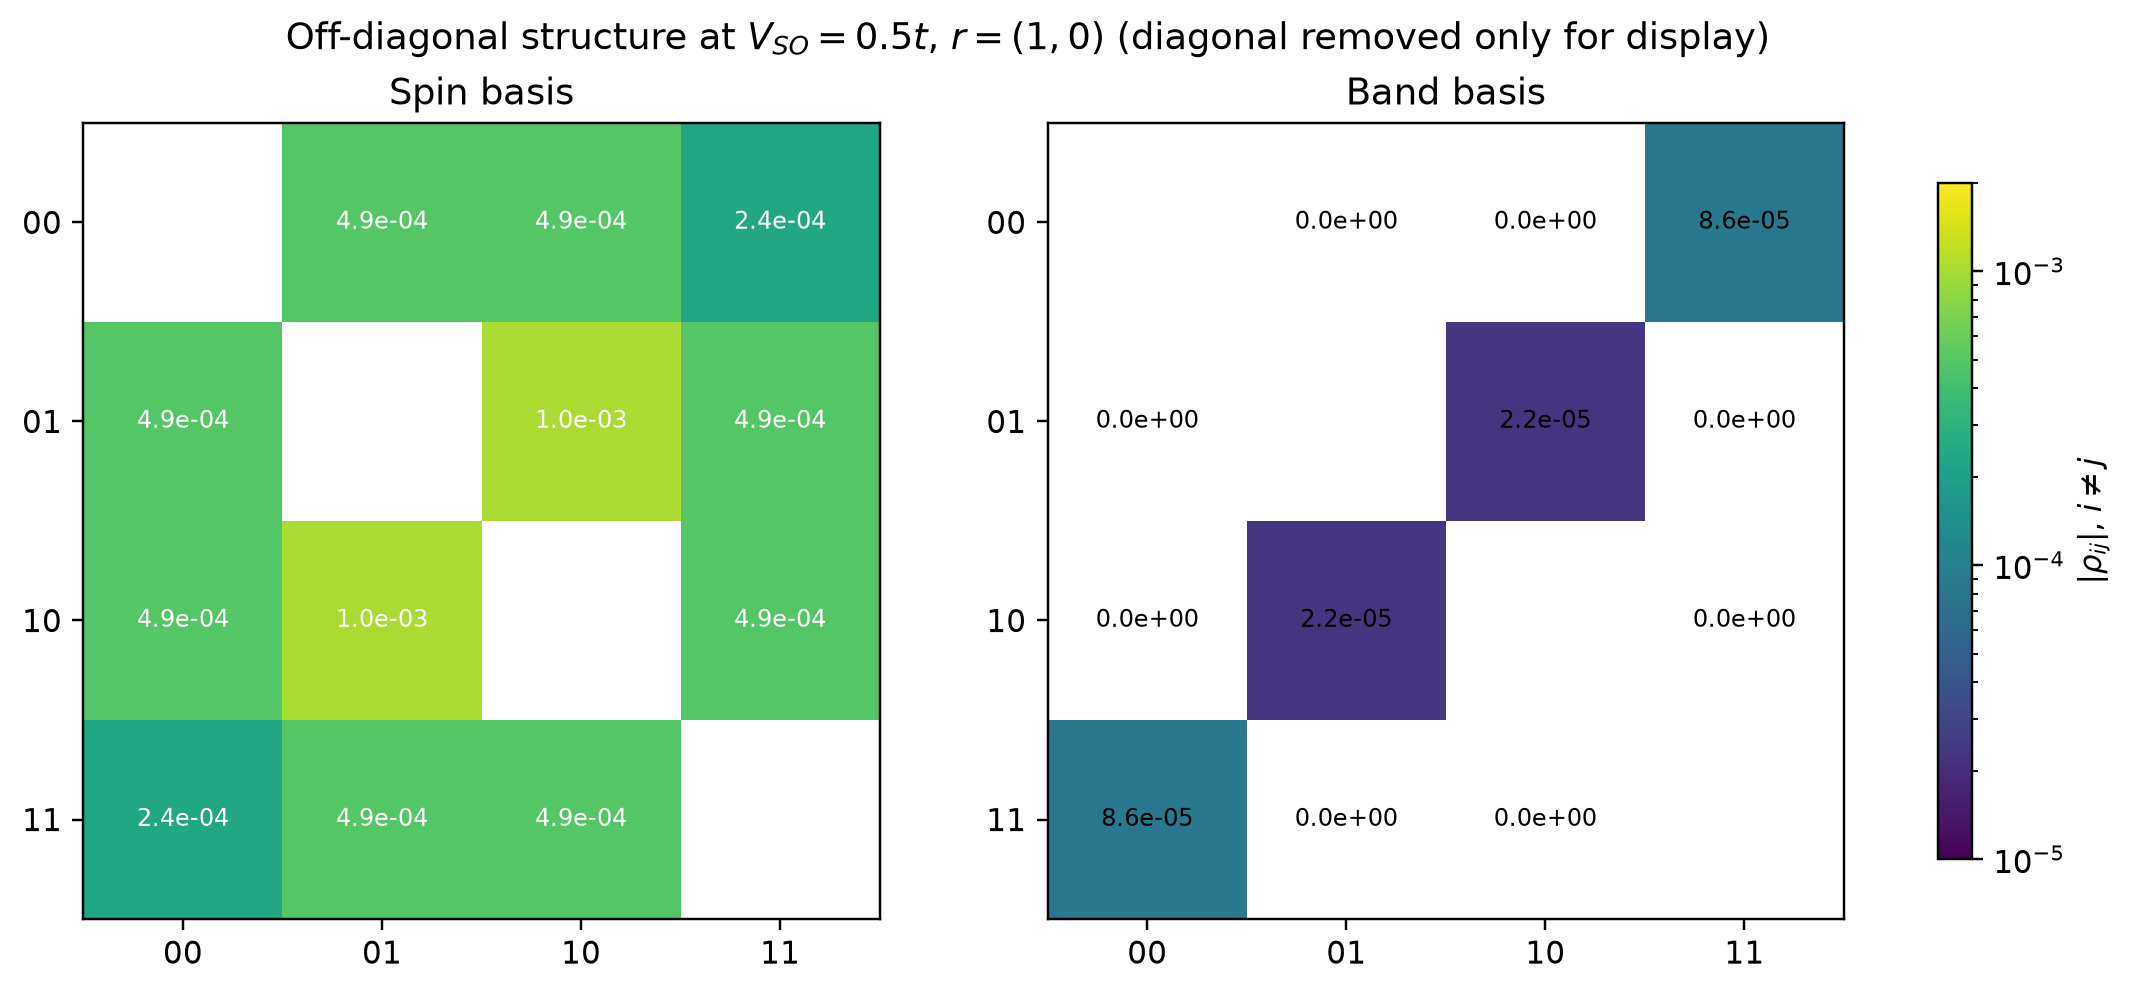
\includegraphics[width=0.95\textwidth]{figs/helicity_density_matrix_offdiagonal.png}
\caption{Off-diagonal magnitudes for the two matrices above. The diagonal is removed only for visualization. Original-spin and band-pseudospin states have different matrix structures and are not interchangeable.}
\label{fig:offdiagonal}
\end{figure}

\subsection{Resource table}

\begin{table}[H]
\centering
\footnotesize
\caption{Validated $\SO=0.5t$ resources at exact lattice vectors. $\Fbar_{\rm ref}$ is fixed-reference teleportation, $\Fbar_{\rm opt}$ is locally optimized average teleportation, and $\chi_{\rm P}$ is the implemented Pauli-ensemble Holevo quantity. No state below the top singlets has an operational advantage.}
Spin & $(0,0)$ & 1.000000000 & 1.000000000 & 1.000000000 & 2.000000000 & 1.000000000 \\
Spin & $(1,0)$ & 0.000000000 & 0.500934644 & 0.501254157 & 0.000013593 & 1.000000000 \\
Spin & $(1,1)$ & 0.000000000 & 0.500576534 & 0.500938408 & 0.000007613 & 1.000000000 \\
Spin & $(2,0)$ & 0.000000000 & 0.500022720 & 0.500371458 & 0.000001194 & 1.000000000 \\
Spin & $(0,2)$ & 0.000000000 & 0.500022720 & 0.500371458 & 0.000001194 & 1.000000000 \\
Spin & $(3,1)$ & 0.000000000 & 0.499980198 & 0.500077918 & 0.000000053 & 1.000000000 \\
Band & $(0,0)$ & 1.000000000 & 1.000000000 & 1.000000000 & 2.000000000 & 1.000000000 \\
Band & $(1,0)$ & 0.000000000 & 0.499739591 & 0.500302714 & 0.002351021 & 0.997651326 \\
Band & $(1,1)$ & 0.000000000 & 0.499758658 & 0.500492092 & 0.002285567 & 0.997715465 \\
Band & $(2,0)$ & 0.000000000 & 0.499455102 & 0.500623183 & 0.002201482 & 0.997798638 \\
Band & $(0,2)$ & 0.000000000 & 0.499455102 & 0.500623183 & 0.002201482 & 0.997798638 \\
Band & $(3,1)$ & 0.000000000 & 0.499486978 & 0.500525833 & 0.002207541 & 0.997792461 \\

\label{tab:resources}
\end{table}

\begin{figure}[H]
\centering
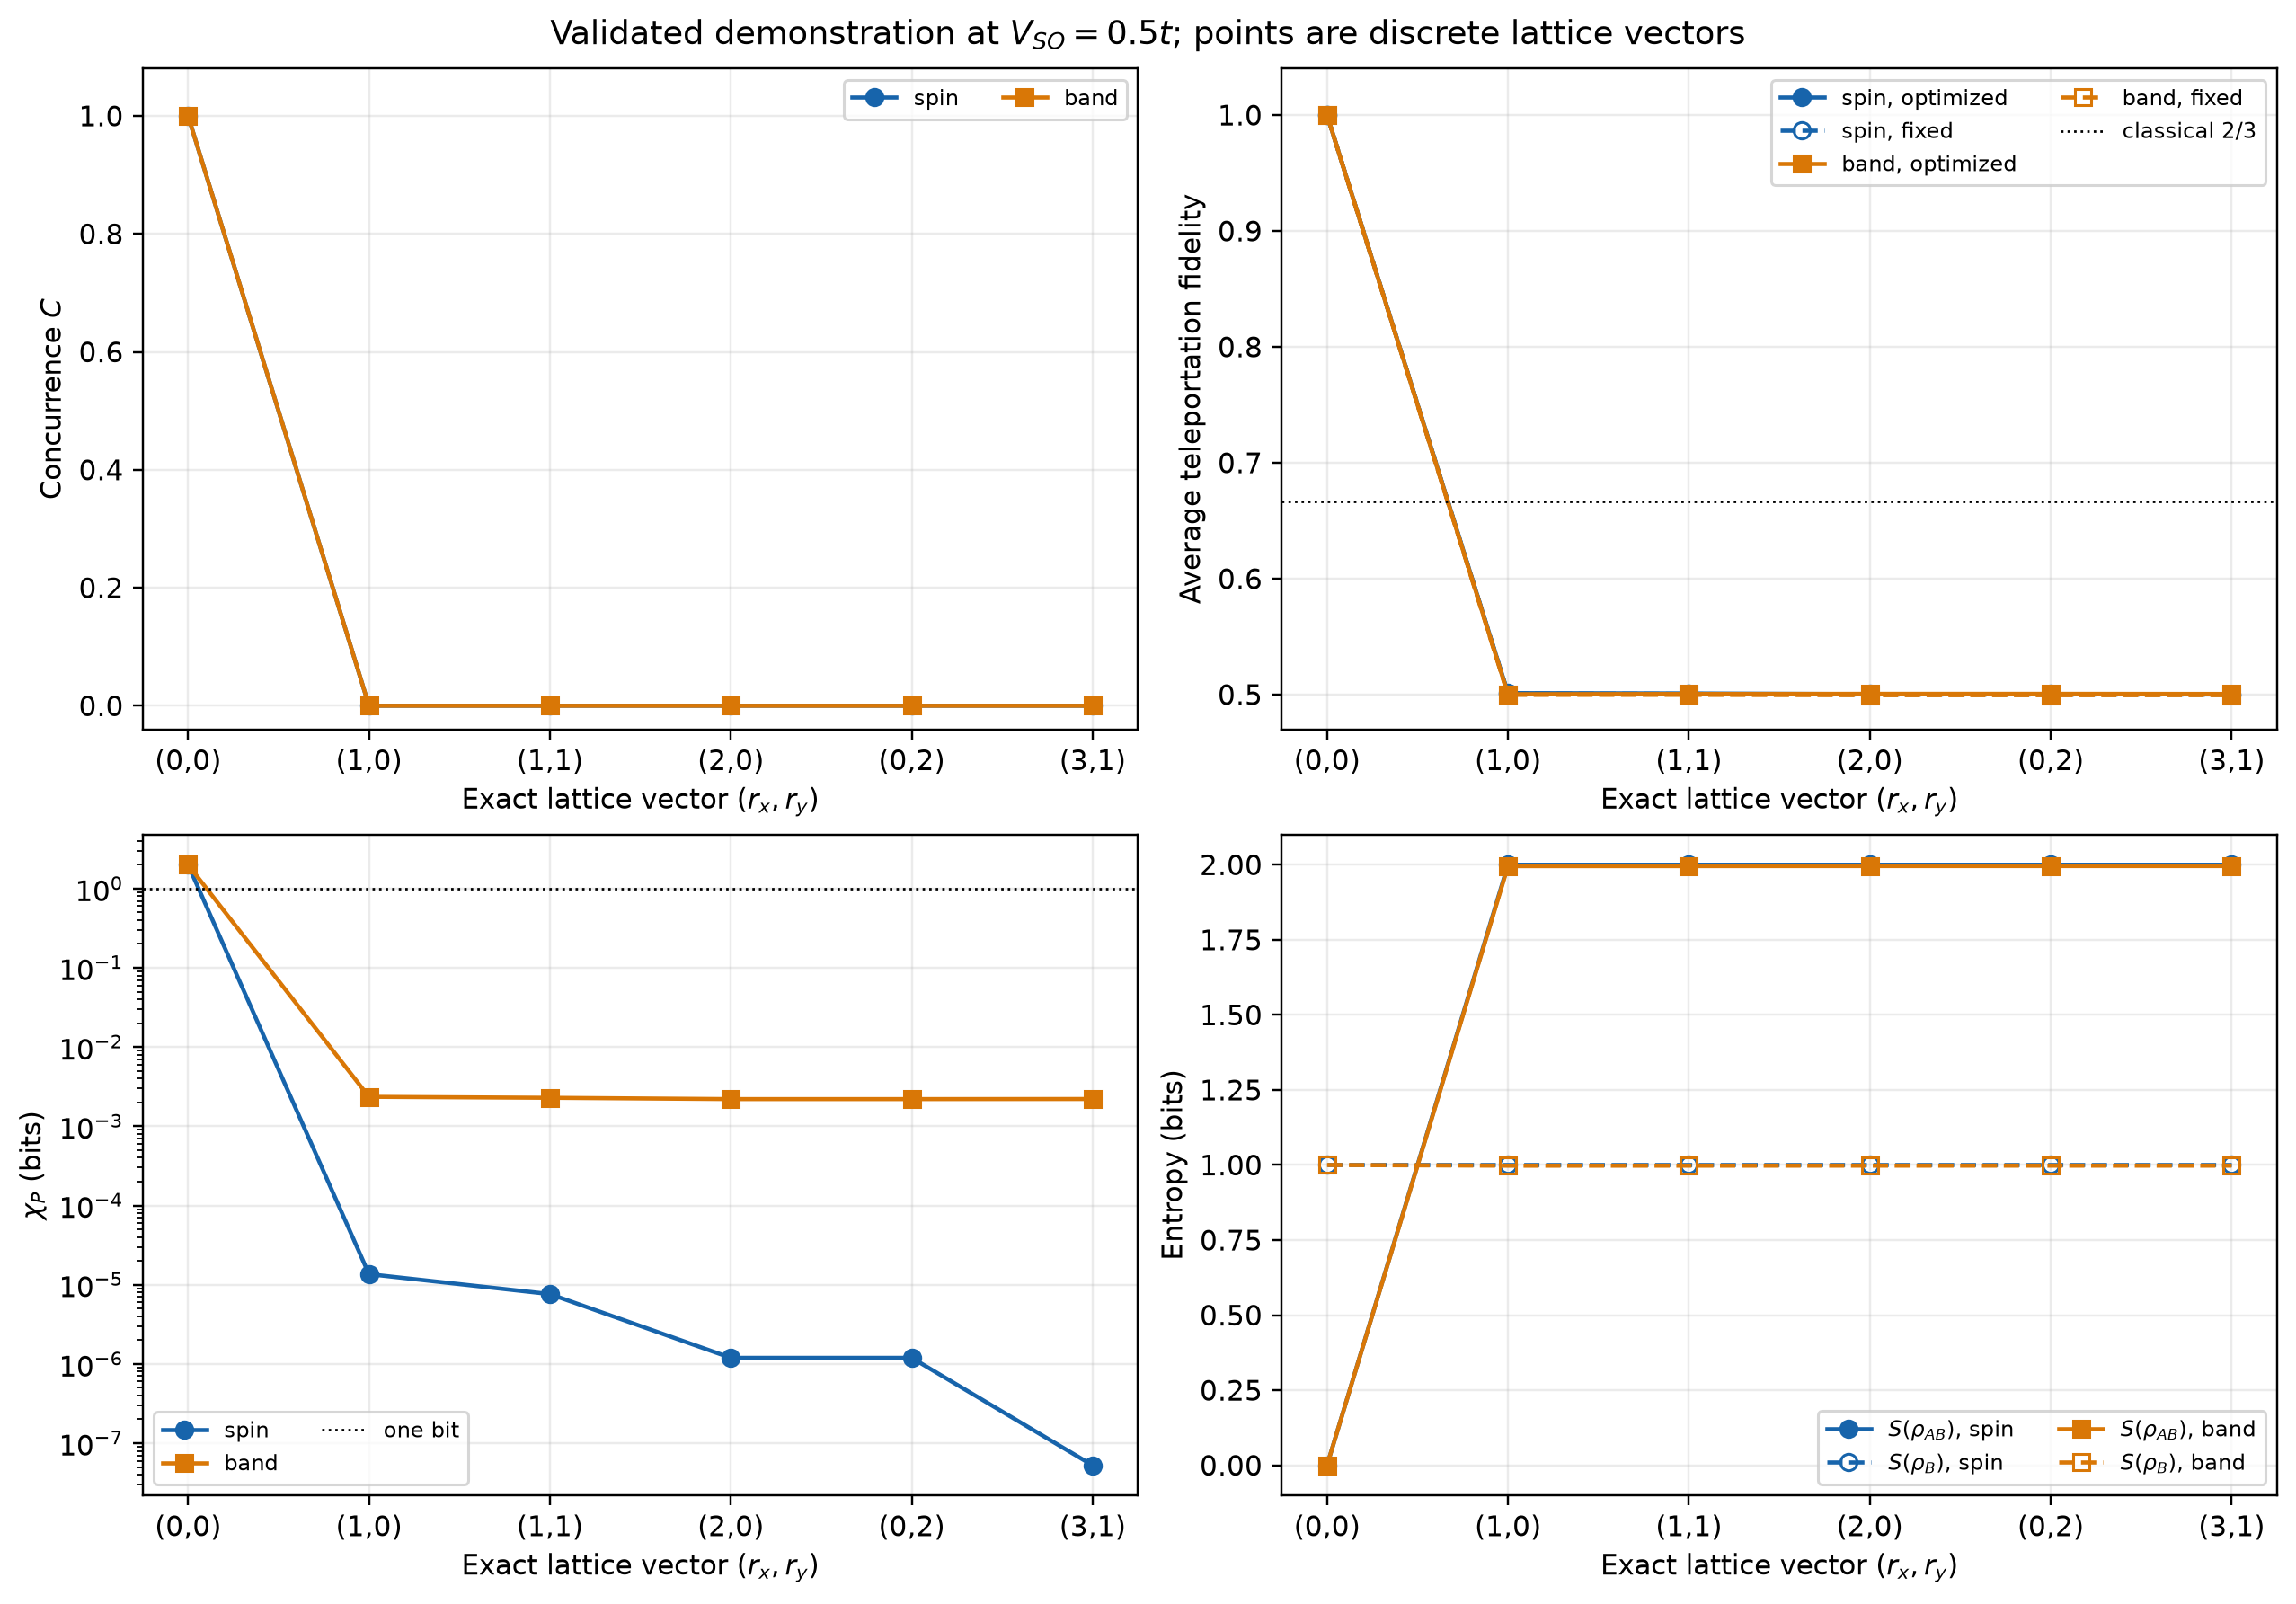
\includegraphics[width=\textwidth]{figs/helicity_density_matrix_resources.png}
\caption{Discrete-lattice resource summary at $\SO=0.5t$. Lines connect discrete points only as visual guides. The same-site singlet has ideal values; all tested nonzero-site states remain below the teleportation and dense-coding benchmarks.}
\label{fig:resources}
\end{figure}

\section{Algorithm and code map}
\label{sec:algorithm}

The implemented algorithm is:
\begin{enumerate}
\item Solve the BdG self-consistency equations for the chosen $U,\Delta_t,n,\SO,N_k,T$.
\item Construct $v_{\kb s}^2$ and $\bar\Delta_{\kb s}/(2E_{\kb s})$.
\item Restore the full phase $s e^{-i\theta_{\kb}}$ and enforce TRIM/Pauli constraints.
\item Build matrix-valued band correlators using Eqs.~\eqref{eq:Nband}--\eqref{eq:Fband}.
\item For original spin, apply Eq.~\eqref{eq:spin_transform}; for band qubits, retain the band matrices.
\item Fourier-transform to $A,B$ using Eq.~\eqref{eq:real_space}.
\item Evaluate all 16 elements with the Wick formula Eq.~\eqref{eq:wick_full}.
\item Retain $P_{AB}$, normalize once, and check trace, Hermiticity, and positivity.
\item Calculate general concurrence, fixed-reference fidelity, FEF, optimized teleportation fidelity, entropies, and $\chi_{\mathrm P}$ separately.
\end{enumerate}

\begin{verbatim}
from helicity_density_matrix import (
    density_at_separation, resource_metrics, dense_coding_metrics)

spin = density_at_separation(bdg, [1, 0], basis="spin")
band = density_at_separation(bdg, [1, 0], basis="band")

print(spin["weight"], resource_metrics(spin["rho"]))
print(dense_coding_metrics(spin["rho"]))
print(band["weight"], resource_metrics(band["rho"]))
print(dense_coding_metrics(band["rho"]))
\end{verbatim}

The main files are:
\begin{itemize}
\item \verb|helicity_density_matrix.py|: correlators, Wick construction, general concurrence, teleportation, and dense-coding metrics;
\item \verb|analysis/validate_helicity_density_matrix.py|: fresh solver runs and validation;
\item \verb|data/helicity_density_matrix_demo.npz|: matrices, correlators, weights, and observables;
\item \verb|reports/helicity_density_matrix_validation.json|: complete diagnostics;
\item \verb|analysis/generate_helicity_report_assets.py|: report tables and figures generated from the NPZ.
\end{itemize}

\section{Scope, limitations, and next calculations}
\label{sec:limitations}

\begin{enumerate}
\item \textbf{Gaussian mean-field scope.} Wick factorization applies to the quadratic BdG state, not automatically to an exact non-Gaussian Hubbard ground state.
\item \textbf{Pairing scope.} The formulas assume spatially uniform zero-center-of-mass-momentum intraband pairing. Interband pairing, FFLO states, disorder, or position-dependent gaps require their full correlators.
\item \textbf{Conditional detection.} The result is not a canonical fixed-total-number reduction of the full BCS state.
\item \textbf{Numerical scope.} Two SOC values and one mesh do not establish a continuous SOC dependence. Production work requires seed and mesh convergence, occupation checks, and independent exact-site evaluation.
\item \textbf{Operational scope.} Band-pseudospin entanglement is not evidence that helicity Bell measurement, local Pauli feedforward, or dense-coding transmission is experimentally available.
\item \textbf{Dynamical scope.} No new environmental evolution is asserted. Noise acts on a specified qubit basis and must be applied to that basis's density matrix.
\item \textbf{No automatic positive result.} A larger gap or anomalous correlator is not, by itself, evidence of teleportation or dense-coding advantage.
\end{enumerate}

The next scientifically useful calculation is a production $\SO$ sweep with independently reconverged BdG solutions, at least two momentum meshes, exact lattice-site resources, and separate original-spin and band-pseudospin labels. Only then should trends with SOC be discussed.

\appendix
\section{Common sign and convention errors}
\label{app:errors}

\begin{itemize}
\item \textbf{Dropping $s e^{-i\theta_{\kb}}$.} This confuses $\bar\Delta_{\kb s}$ with the full gap and violates the required pair structure.
\item \textbf{Using $UNU^\dagger$ blindly.} For $N_{\sigma\sigma'}=\langle c_\sigma^\dagger c_{\sigma'}\rangle$, the implemented spin transformation is $U^*NU^T$.
\item \textbf{Using $U_{\kb}$ for both anomalous operators.} The pair has momenta $\kb,-\kb$, so the transformation contains $U_{\kb}F_{\kb}U_{-\kb}^T$.
\item \textbf{Ignoring TRIM points.} Nondegenerate same-band pairing vanishes where the two time-reversed operators coincide.
\item \textbf{Using $F_{BA}^*$ with the wrong sign.} The creation-side factor in the Wick matrix is $F_{AB,\alpha'\beta'}^*=-F_{BA,\beta'\alpha'}^*$.
\item \textbf{Forgetting same-site antisymmetry.} $F_{AB}(0)$ must be antisymmetric; finite-grid residue is not a physical same-spin onsite pair.
\item \textbf{Projecting onto an $X$ state.} This hides precisely the new SOC-generated matrix elements.
\item \textbf{Clipping negative eigenvalues.} Positivity must follow from the physical contraction; clipping would conceal implementation errors.
\item \textbf{Equating spin and band protocols.} The Pauli algebra is identical, but the physical modes and required operations differ.
\end{itemize}

\section{Reproducibility}
\label{app:repro}

From the repository root:
\begin{verbatim}
.venv/bin/python analysis/validate_helicity_density_matrix.py
.venv/bin/python analysis/generate_helicity_report_assets.py
\end{verbatim}
The validation writes only helicity-specific artifacts and does not overwrite archived $\SO=0$ Green's-function files. The report assets script reads the validated NPZ and generates every numerical table and both report figures. The PDF is compiled independently of \verb|manuscript.pdf|.

\begin{thebibliography}{99}

\bibitem{Hutchinson2018}
J. Hutchinson, J. E. Hirsch, and F. Marsiglio,
\emph{Enhancement of superconducting $T_c$ due to the spin-orbit interaction},
Phys. Rev. B \textbf{97}, 184513 (2018),
\href{https://arxiv.org/html/1801.08988}{arXiv:1801.08988}.

\bibitem{Oh2005}
S. Oh and J. Kim,
\emph{Entanglement of electron spins in superconductors},
Phys. Rev. B \textbf{71}, 144523 (2005),
\href{https://arxiv.org/pdf/quant-ph/0406013}{arXiv:quant-ph/0406013}.

\bibitem{Wootters1998}
W. K. Wootters,
\emph{Entanglement of formation of an arbitrary state of two qubits},
Phys. Rev. Lett. \textbf{80}, 2245 (1998).

\bibitem{Bennett1993}
C. H. Bennett, G. Brassard, C. Cr\'epeau, R. Jozsa, A. Peres, and W. K. Wootters,
\emph{Teleporting an unknown quantum state via dual classical and Einstein-Podolsky-Rosen channels},
Phys. Rev. Lett. \textbf{70}, 1895 (1993).

\bibitem{Horodecki1999}
M. Horodecki, P. Horodecki, and R. Horodecki,
\emph{General teleportation channel, singlet fraction, and quasidistillation},
Phys. Rev. A \textbf{60}, 1888 (1999).

\bibitem{BennettWiesner1992}
C. H. Bennett and S. J. Wiesner,
\emph{Communication via one- and two-particle operators on Einstein-Podolsky-Rosen states},
Phys. Rev. Lett. \textbf{69}, 2881 (1992).

\bibitem{Bruss2004}
D. Bru\ss, G. M. D'Ariano, M. Lewenstein, C. Macchiavello, A. Sen(De), and U. Sen,
\emph{Distributed quantum dense coding},
Phys. Rev. Lett. \textbf{93}, 230501 (2004).

\end{thebibliography}

\end{document}
